% ---------------------------------------------------------------------------
% Chapter -- Oscillating Control Design
% The controller is the r = 3 truncation of eq. (16) of
% Zuyev & Grushkovskaya, arXiv:2403.03341, Sec. IV.
% The paper proves convergence for r = 4 only (see Section 5.5).
% Figure: code/fig_one_period.py -> figures/fig_one_period.pdf
% ---------------------------------------------------------------------------

\chapter{Oscillating Control Design}
\label{ch:control}
\TODO[status of this chapter: text rewritten; two open questions for the supervisor, see the TODOs in 5.4 and 5.5]

Chapter~\ref{ch:model} showed that no continuous feedback that depends only on
the state can stabilize the car with trailers. Chapter~\ref{ch:nilpotent}
replaced the model by a simpler system, the nilpotent approximation
$\dot z=u_1g_1(z)+u_2g_2(z)$. This chapter designs a controller for that system,
and the controller depends on time. The approach comes
from~\cite{zuyev2016,grushkovskaya2023}, and it was applied to off-hooked
trailers in~\cite{zuyev2024}. The inputs oscillate, and the oscillations move
the system in the directions that the two inputs cannot reach directly. For the
car with one trailer, the controller is a shortened version of the controller
from~\cite{zuyev2024}: it is cut after the second bracket ($r=3$).
\Cref{sec:convergence} says what is proved for it and what is not.

% ===========================================================================
\section{Idea}
\label{sec:idea}

Take the nilpotent system $\dot z=u_1g_1(z)+u_2g_2(z)$ with the matrix $G(z)$
from \cref{sec:approx1}. Suppose that all four coordinates could be moved
independently. This would mean a ``virtual'' input $v$ with four components, so
that $\dot z=G(z)v$, and $v$ could be chosen so that $z$ moves toward the goal.
The real system has only two inputs. But the oscillating inputs defined below
give, over one period $\varepsilon$, the displacement
\begin{equation}
  z(\varepsilon)\approx z(0)+\varepsilon\,G(z)\,a(z),
  \label{eq:step}
\end{equation}
where $a=(a_1,a_2,a_{12},a_{112})^\top$ is a vector of four amplitudes that can
be chosen freely. The amplitudes $a_1$ and $a_2$ move the coordinates that are
reached directly. The amplitudes $a_{12}$ and $a_{112}$ move the coordinates that
are reached through the first and the second Lie bracket. This is why the indices
are the brackets written as digits. The formula is made exact in
\cref{sec:convergence}.

Next, a function $V(z)$ is chosen that measures how far $z$ is from the goal. It
is zero at the goal and positive everywhere else. It is called a Lyapunov
function. The amplitudes are chosen as
\begin{equation}
  a(z)=-G(z)^{-1}\nabla V(z).
  \label{eq:agradient}
\end{equation}
Then $G(z)a(z)=-\nabla V(z)$, and \eqref{eq:step} becomes
\begin{equation}
  z_{j+1}\approx z_j-\varepsilon\nabla V(z_j).
\end{equation}
This is one step of gradient descent with step length $\varepsilon$: the state
moves a little in the direction in which $V$ decreases fastest. For small steps,
this is the gradient flow $\dot z=-\nabla V(z)$. This is the core of the method:
\emph{one period of the oscillating controller is one step of gradient descent
in the privileged coordinates.} The inverse $G(z)^{-1}$ exists for every $z$,
because $\det G(z)=1$ \eqref{eq:detG}, so this choice is always possible.

\paragraph{Radial Lyapunov functions.}
In this thesis, $V$ depends only on the distance $r=\|z\|$ to the goal:
$V(z)=\Phi(r)$. Then $\nabla V(z)=(\Phi'(r)/r)\,z$. It is convenient to write this
as $\nabla V(z)=\gamma\,h(z)\,z$, so that
\begin{equation}
  a(z)=-\gamma\,h(z)\,G(z)^{-1}z,\qquad h(z)=\frac{\Phi'(r)}{\gamma r}.
  \label{eq:ah}
\end{equation}
The constant $\gamma>0$ is called the gain. The function $h$ is the only place
where the choice of $V$ enters the controller. Three choices are used:
\begin{center}
\begin{tabular}{lll}
  \toprule
  $V$ & $\Phi(r)$ & $h(z)$ \\
  \midrule
  quadratic & $\gamma r^2/2$ & $1$ \\
  logarithmic & $\dfrac{\gamma}{2c}\ln(1+cr^2)$ & $\dfrac{1}{1+c\,r^2}$ \\[6pt]
  square-root & $\gamma\bigl(\sqrt{r^2+\delta^2}-\delta\bigr)$ & $\dfrac{1}{\sqrt{r^2+\delta^2}}$ \\
  \bottomrule
\end{tabular}
\end{center}
They differ in how the length of the step depends on the distance to the goal.
Their effect on the speed of convergence is compared in
Chapter~\ref{ch:feasibility}.
For the car with one trailer, $G(z)$ is lower triangular, and \eqref{eq:ah}
gives
\begin{equation}
  \begin{aligned}
  a_1&=-\gamma h\,z_1, & a_{12}&=-\gamma h\,(z_1z_2+z_3),\\
  a_2&=-\gamma h\,z_2, & a_{112}&=-\gamma h\,(\alpha z_2^{3}+z_1z_3+z_4).
  \end{aligned}
  \label{eq:amps}
\end{equation}
Each amplitude is large when the coordinate it belongs to is far from zero. The
extra terms, such as $z_1z_2$ in $a_{12}$, are needed because the directions
$g_1,g_2,\dots$ influence each other's coordinates. For example, moving $z_1$ and
$z_2$ also changes $z_3$.

\begin{figure}[t]
  \centering
  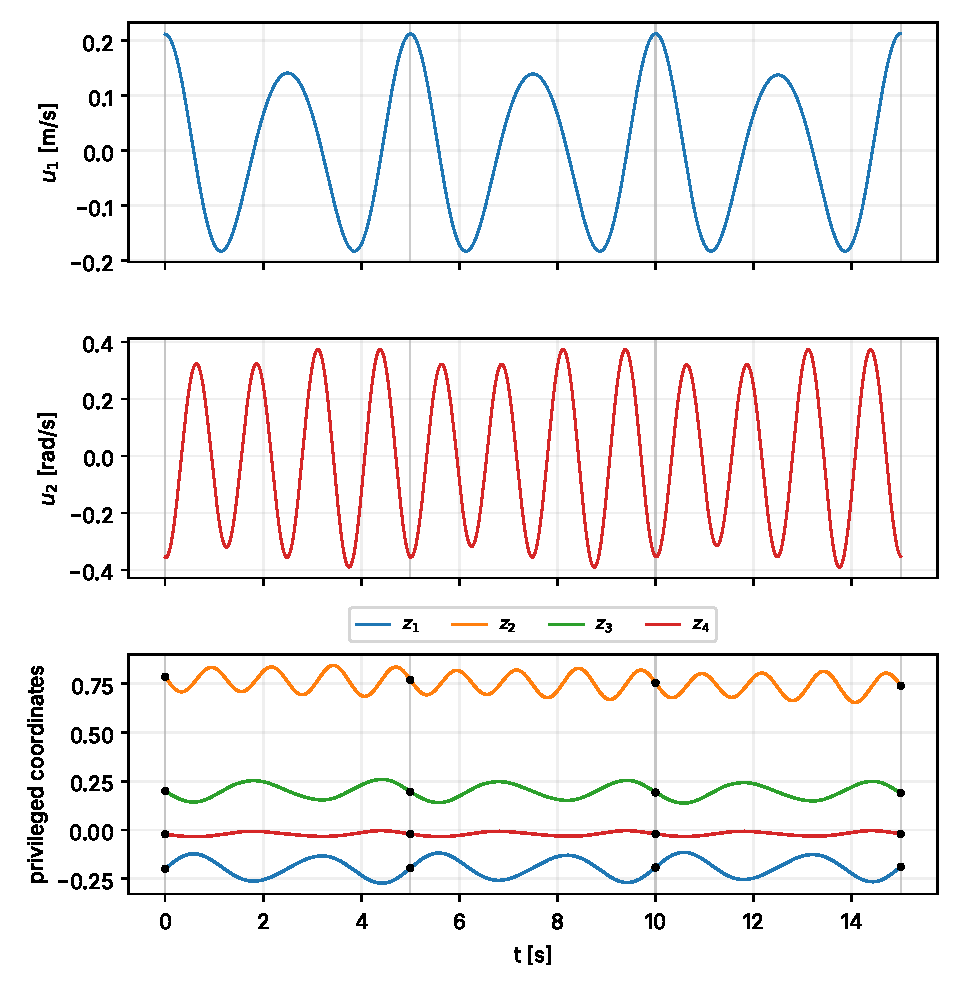
\includegraphics[width=0.78\textwidth]{fig_one_period.pdf}
  \caption{The controller over three sampling intervals (one trailer, platform
  lengths, $\varepsilon=\SI{5}{s}$, $(k_{12},k_{112})=(3,2)$,
  $\|z(0)\|=0.835$). Top and middle: the inputs $u_1$ and $u_2$. Bottom: the
  privileged coordinates. The dots mark the start of each interval. Within an
  interval, the coordinates swing back and forth. Over a full period, the net
  movement is the small gradient step \eqref{eq:step}.}
  \label{fig:oneperiod}
\end{figure}

% ===========================================================================
\section{Controller structure}
\label{sec:structure}

The controller has a constant part and one oscillating term for each level of
Lie brackets. Let $\omega=2\pi/\varepsilon$. For $r=3$, the controller is
\begin{align}
  u_1&=a_1+T_{12}\cos(k_{12}\omega t)+T_{112}\cos(k_{112}\omega t),\\
  u_2&=a_2+T_{12}\,\mathrm{sign}(a_{12})\sin(k_{12}\omega t)
        -2T_{112}\,\mathrm{sign}(a_{112})\cos(2k_{112}\omega t),
  \label{eq:controller}
\end{align}
with the sizes
\begin{equation}
  T_{12}=\bigl(2k_{12}\omega\,|a_{12}|\bigr)^{1/2},\qquad
  T_{112}=(2k_{112}\omega)^{2/3}\,|a_{112}|^{1/3}.
  \label{eq:Tsizes}
\end{equation}
The integers $k_{12}$ and $k_{112}$ are the frequency multipliers
(\cref{sec:multipliers}). The amplitudes $a_1,a_2,a_{12},a_{112}$ are given
by \eqref{eq:amps}. The inputs $u_1$ and $u_2$ are the physical driving speed and
turning speed of the robot.

\paragraph{Why these amplitudes.}
The second level is taken first. Let $u_1=T\cos\theta$ and $u_2=Ts\sin\theta$,
where $\theta=k_{12}\omega t$ and $s=\pm1$. Integrating $u_2$ gives
$z_2(t)=z_2(0)+\frac{Ts}{k_{12}\omega}(1-\cos\theta)$. The third equation,
$\dot z_3=-z_2u_1$, then has the mean value over one period
\begin{equation}
  \overline{\dot z_3}=-\frac{T^2s}{k_{12}\omega}\;\overline{(1-\cos\theta)\cos\theta}
  =\frac{T^2s}{2k_{12}\omega}.
\end{equation}
The term $z_2(0)\cos\theta$ averages to zero. Setting the mean equal to $a_{12}$
gives $T^2=2k_{12}\omega|a_{12}|$ and $s=\mathrm{sign}\,a_{12}$. This is $T_{12}$
in \eqref{eq:Tsizes}. So the oscillation produces a steady drift in $z_3$,
although neither input moves $z_3$ directly. This is the parking effect: a closed
manoeuvre of the two inputs leaves a net movement in a direction that neither
input moves directly.

For the third level, let $u_1=T\cos\theta$ and $u_2=-2Ts\cos2\theta$, where
$\theta=k_{112}\omega t$. Then $z_3$ oscillates, but it returns to its starting
value after one period. So the first bracket produces no net movement, and the
mean of $\dot z_4=-z_3u_1-\alpha z_2^2u_2$ is
\begin{equation}
  \overline{\dot z_4}=\frac{T^3s}{4k_{112}^2\omega^2}.
\end{equation}
The term $\alpha z_2^2u_2$ averages to zero. Setting the mean equal to $a_{112}$
gives $T^3=4k_{112}^2\omega^2|a_{112}|$. This is $T_{112}$ in
\eqref{eq:Tsizes}. Both computations were checked symbolically
(\cref{app:control}).

\paragraph{Cost of the deep brackets.}
A bracket of length $k$ needs an oscillation of size
$T\propto\omega^{(k-1)/k}|a|^{1/k}$, because the displacement it produces is of
order $T^k/\omega^{k-1}$. This gives the powers $\omega^{1/2}$ and $\omega^{2/3}$
for $r=3$. For the car with two trailers there is one more power, $\omega^{3/4}$.
The controller from~\cite{zuyev2024} then has a third oscillating term,
\begin{equation}
  2\bigl(k_{1112}\omega\bigr)^{3/4}|a_{1112}|^{1/4}\cos(k_{1112}\omega t)
\end{equation}
in $u_1$ and $-6(k_{1112}\omega)^{3/4}|a_{1112}|^{1/4}\,\mathrm{sign}(a_{1112})\sin(3k_{1112}\omega t)$
in $u_2$. So the deepest bracket costs the most control effort. This is why one
trailer is much easier to control than two. The numbers are in
Chapter~\ref{ch:feasibility}.

% ===========================================================================
\section{Sampling scheme}
\label{sec:sampling}

The amplitudes depend on the state, but they are not updated all the time. On
each interval $[j\varepsilon,(j+1)\varepsilon)$, they are computed from the state
at the start of the interval, $z_j=z(j\varepsilon)$, and kept constant:
\begin{equation}
  u(t)=u\bigl(t;z_j\bigr),\qquad t\in[j\varepsilon,(j+1)\varepsilon).
\end{equation}
So $\varepsilon$ is both the period of the oscillations
($\omega=2\pi/\varepsilon$) and the time between two updates. Trajectories made
in this way are called $\pi_\varepsilon$-solutions in~\cite{zuyev2024}. Since
$k\omega\varepsilon=2\pi k$ for an integer $k$, it does not matter whether $t$ in
\eqref{eq:controller} is the absolute time or the time since the start of the
interval.

Only the state is converted between the physical coordinates $x$ and the
privileged coordinates $z$. This is done once at the start of each interval, with
\eqref{eq:xtoz1} (or \eqref{eq:xtoz2} for two trailers). The inputs need no
conversion, because $u_1$ and $u_2$ are the driving speed and the turning speed of
the robot in both descriptions. On the TurtleBot, $u_1$ is sent as the linear
velocity and $u_2$ as the angular velocity of the velocity command. In ROS~2 this
is a message of type \texttt{geometry\_msgs/Twist} on the topic
\texttt{/cmd\_vel}, with $u_1$ in the field \texttt{linear.x} and $u_2$ in
\texttt{angular.z}.

% ===========================================================================
\section{Choice of frequency multipliers}
\label{sec:multipliers}

The multipliers $k_{12}$ and $k_{112}$ are positive integers. With integers, every
oscillating term completes whole periods during one interval. So the
oscillations by themselves leave no net movement in the directions $z_1$ and
$z_2$.

\paragraph{Non-resonance.}
The multipliers must also avoid resonances between the different terms. A
resonance means that the frequencies are related by a simple whole-number
relation, so that the terms can combine into an unwanted net movement. Following
\cite{zuyev2024}, a tuple $(k_1,\dots,k_s)$ is called \emph{resonant of order $K$}
if there are integers $c_1,\dots,c_s$ with no common divisor larger than $1$, with
$\sum|c_i|=K$ and $\sum c_ik_i=0$. For $r=4$, the paper requires that the tuples
$(k_{12},k_{112},k_{1112})$, $(k_{12},2k_{112},k_{1112})$,
$(k_{12},k_{112},3k_{1112})$ and $(k_{12},2k_{112},3k_{1112})$ have no resonance
of order up to $4$ (condition C1). This condition is stated for three
multipliers. For $r=3$ there are only two, and the paper does not say which
condition they have to satisfy.

\paragraph{What the computation shows.}
For the nilpotent system, the effect of a resonance can be seen directly. One
interval was integrated with $a_1=a_2=0$, for all pairs with
$1\le k_{12},k_{112}\le12$ and for all sign combinations of $a_{12}$ and
$a_{112}$ (\cref{app:control}). In every case, the displacement equals
$\varepsilon\,(0,0,a_{12},a_{112})^\top$ up to numerical accuracy. The exceptions
are the pairs with
\begin{equation}
  k_{12}=k_{112}\qquad\text{or}\qquad k_{12}=3\,k_{112}.
  \label{eq:resonant}
\end{equation}
For these, an unwanted term appears in $z_4$. It is proportional to
$\sqrt{|a_{12}|}\,|a_{112}|^{2/3}\varepsilon^{7/6}$. A plausible reason for the
second case is the following. The input $u_1$ contains the frequency $k_{112}$,
and $u_2$ contains $2k_{112}$. The third-order terms combine three oscillations,
so the $k_{12}$ term can resonate with them when $k_{12}=k_{112}+2k_{112}$. This
is a computation for the approximating system, and not a proof of convergence.
But it shows which pairs have to be avoided.

The pair used in this thesis, $(k_{12},k_{112})=(3,2)$, is not one of these
cases. In the MATLAB code, the pairs are screened with a stricter practical rule:
neither multiplier may be an integer multiple of the other. The pair $(3,2)$ came
out on top of the ranking made by the search. This rule is not the condition
from~\cite{zuyev2024}. It excludes pairs, such as $(2,1)$, for which no unwanted
term was found.
\TODO[Ask the supervisor which non-resonance condition applies for two multipliers, and whether the computed result above could be stated as a lemma]

% ===========================================================================
\section{Convergence}
\label{sec:convergence}

\paragraph{One interval.}
For the nilpotent system the equations are triangular, so the integral over one
interval can be computed exactly. This was done by computer algebra
(\cref{app:control}), for the multipliers $(3,2)$ and amplitudes kept constant at
$z$. The result is the following.

\begin{lemma}
\label{lem:interval}
Let $z(\cdot)$ be the solution of $\dot z=u_1g_1(z)+u_2g_2(z)$ from
\eqref{eq:nilp1} with the controls \eqref{eq:controller},
$(k_{12},k_{112})=(3,2)$, and amplitudes kept constant at $z(0)=z$. Then
\begin{equation}
  z(\varepsilon)=z+\varepsilon\,G(z)\,a(z)+R,\qquad
  G(z)a(z)=\begin{pmatrix}a_1\\ a_2\\ a_{12}-z_2a_1\\ a_{112}-z_3a_1-\alpha z_2^2a_2\end{pmatrix},
  \label{eq:interval}
\end{equation}
where $R_1=R_2=0$, the third component is
\begin{equation}
  R_3=-\tfrac12\varepsilon^{2}a_1a_2-\mathrm{sign}(a_{12})\,a_1\,\varepsilon^{3/2}\sqrt{\frac{|a_{12}|}{3\pi}},
\end{equation}
and every term of $R_4$ contains $a_1$ or $a_2$. In particular, $R=0$ if
$a_1=a_2=0$.
\end{lemma}

So the displacement is the ideal step \eqref{eq:step} plus a remainder $R$. The
remainder is zero when the constant parts $a_1$ and $a_2$ are zero. The first two
coordinates are moved exactly.

\paragraph{The contraction.}
With $a=-\gamma hG^{-1}z$, the ideal step is $G(z)a(z)=-\gamma h(z)\,z$, so
\begin{equation}
  z_{j+1}=(1-\mu_j)\,z_j+R_j,\qquad \mu_j=\varepsilon\,\gamma\,h(z_j).
  \label{eq:contraction}
\end{equation}
For $z_1$ and $z_2$ this holds without a remainder:
$z_{1,j+1}=(1-\mu_j)z_{1,j}$. If the remainder is small compared with
$\mu_j\|z_j\|$, the norm decreases by the factor $1-\mu_j$ in every interval.
This means that it converges geometrically, and the rate is set by
$\varepsilon\gamma h$. This is the role of $\gamma$: it sets the rate of
convergence, and it is limited from above by the velocity limits of the robot
(Chapter~\ref{ch:feasibility}).

The size of the remainder depends on the single number
$\mu=\varepsilon\gamma h$. For the platform lengths and the start state $z_0$ of
the experiment, the computed size of $R$ relative to the step is:
\begin{center}
\begin{tabular}{rrr}
  \toprule
  $\mu=\varepsilon\gamma h(z_0)$ & $\gamma$ & $\|R\|/\|\varepsilon G a\|$ \\
  \midrule
  0.005 & $8.0\times10^{-4}$ & 0.0017\\
  0.019 & $3.2\times10^{-3}$ & 0.0045\\
  0.077 & $1.3\times10^{-2}$ & 0.0125\\
  0.153 & $2.6\times10^{-2}$ & 0.0218\\
  \bottomrule
\end{tabular}
\end{center}
The remainder is small, and it gets smaller compared with the step as $\mu$ gets
smaller. In the gain selection used in the code, the product $\varepsilon\gamma h$
is also capped ($\le0.8$), so that the factor $1-\mu$ never changes sign.

\paragraph{Continuous-time view.}
The sampled motion approximately follows the gradient flow
$\dot z=-\nabla V(z)$. For a $V$ that depends only on the distance, the distance
$r=\|z\|$ obeys $\dot r=-\Phi'(r)$. The time to reach a fraction $q$ of the
starting distance is
\begin{equation}
  t_q=\int_{q\,r_0}^{r_0}\frac{\mathrm dr}{\Phi'(r)} .
\end{equation}
For the quadratic $V$ this is $t_q=\ln(1/q)/\gamma$, which is exponential
convergence. The other choices of $h$ change how the distance decreases.
Chapter~\ref{ch:feasibility} compares them.

\paragraph{What is proved and what is not.}
For the car with \emph{two} trailers ($r=4$, three multipliers satisfying C1),
\cite{zuyev2024} proves exponential convergence for sufficiently small
$\varepsilon$ (Theorem~1 there). The theorem is about the nilpotent
approximation, and not about the exact system. The proof uses an estimate
$z(\varepsilon)=z+\varepsilon G a+O(\varepsilon^{4/3})$ of the same kind as
\eqref{eq:interval}. The controller for one trailer is the same controller, cut
after the second bracket. Lemma~\ref{lem:interval} gives the corresponding
one-interval result for it, and it shows that the structure of the argument
carries over. But a complete proof of convergence for $r=3$ is not given here,
and it is not claimed that Theorem~1 of~\cite{zuyev2024} covers this case as
stated. For one trailer, the convergence is therefore supported by
Lemma~\ref{lem:interval}, by the simulations in Chapter~\ref{ch:simulation},
and by the experiments in Chapter~\ref{ch:experiments}.
\TODO[Ask the supervisor whether the r=3 convergence should be stated as a remark (as here), a conjecture, or a short proof; and how to cite her confirmation of the controller shape]
